\documentclass[]{beamer}
\usepackage{tikz,lstautogobble,listings}
\usetikzlibrary{arrows.meta}
\usetheme{Rochester}
\usepackage[T1]{fontenc}
\usepackage[utf8]{inputenc}
\lstset{
  language=caml,
  basicstyle=\ttfamily\tiny,
  breaklines=true,
  autogobble=true,
}


\title{TIPE 25/26 - Cycles et Boucles}
\author{GIL Dorian}
\subtitle{Méthode des tableaux : Optimisation et étude de la satisfiabilité de formule}
\date{}

\begin{document}

\begin{frame}
\titlepage
\end{frame}

\begin{frame}{Sommaire}
\begin{enumerate}
    \item Introduction Générale et Objectifs
    \item Etude Introductive: Forme Alternée
    \item Etude dans le cadre de la logique temporelle linéaire
\end{enumerate}
\end{frame}

\begin{frame}{Introduction - Definition}
    \begin{definition}[Méthode des tableaux]
        Algorithme pour prouver qu'une assertion $\phi$ ayant pour hypothèse $(H_n)$ soit satisfiable
    \end{definition}
    On supposera que aucune hypothèse n'est faite, on peut facilement adapter l'étude que l'on va faire lors d'ajout d'hypothèse.
    \pause
    \begin{itemize}
        \item On place $\phi$ et ses hypothèses dans la racine.
        \item On applique des règles $(R_x)$ à chaque formule en bout d'arbre qui sont developpables
        \item Si on trouve des contradictions (des \textit{cycles}) dans toutes les branches de l'arbre (branches fermées), l'arbre est fermé donc la formule est insatisfiable.
    \end{itemize}
    \pause
    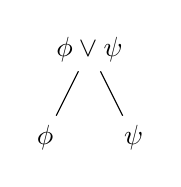
\begin{tikzpicture}[scale=0.75]
    \node {$\phi\lor\psi$}
        child {node {$\phi$}}
        child {node {$\psi$}};
    \end{tikzpicture}
    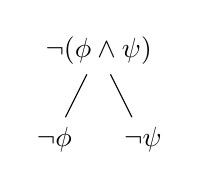
\begin{tikzpicture}[scale=0.75]
    \node {$\lnot(\phi\land\psi)$}
        child {node {$\lnot\phi$}}
        child {node {$\lnot\psi$}};
    \end{tikzpicture}
    \begin{tikzpicture}[scale=0.75]
    \node {$\lnot\lnot\phi$}
        child {node {$\phi$}};
    \end{tikzpicture}
    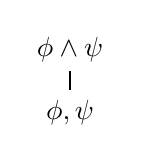
\begin{tikzpicture}[level distance=8mm]
    \node {$\phi\land\psi$}
        child {node {$\phi, \psi$}};
    \end{tikzpicture}  
    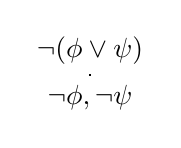
\begin{tikzpicture}[level distance=8mm,scale=0.75]
    \node {$\lnot(\phi\lor\psi)$}
        child {node {$\lnot\phi, \lnot\psi$}};
   \end{tikzpicture}
\end{frame}


\begin{frame}{Introduction - Definition}
    Les règles définis précedemment sont dites Smullyan-Style

    \begin{definition}[Branche fermée]
        Une branche est fermée si elle contient $\phi$ et $\lnot\phi$
    \end{definition}
    Une formule est insatisfisable ssi son arbre associé est dit fermé ssi toutes les branches le sont.
\end{frame}

\begin{frame}{Introduction - Remarques}
    \begin{itemize}
        \item On peut utiliser la méthode des tableaux pour montrer qu'une formule est une tautologie:
        \begin{enumerate}
            \item On place $\lnot\phi$ et ses hypothèses dans la racine.
            \item On applique des règles $(R_x)$ à chaque formule en bout d'arbre qui sont developpables
            \item Si on trouve $a$ et $\lnot a$ dans les branches de l'arbre (des \textit{cycles}), alors $\phi$ est une tautologie
        \end{enumerate}
        On pourra donc aussi adapter nos recherches pour la recherche de tautologie.
        
        \item Nous allons maintenant introduire un type de formule et étudier la méthode des tableaux sur ce cas particulier, pour en déduire des propriétés interessantes.
        Ou même des optimisations de cette méthode.
    \end{itemize}
\end{frame}

\begin{frame}{Alternée - Definition}
    \begin{definition}[Forme Alternée]
        Soit $n\in\mathbb{N}^*$, et $(a_k)_{k\in [|1,n|]}$ des litteraux, on dit que $\varphi$ est de forme alternée ssi
        $$\varphi = a_1\land(a_2\lor(a_3\land(\dots(a_n))))$$
    \end{definition}
    \pause
    On remarquera le parenthesage qui enlève toute ambiguité sur la prioritée entre les opérateurs logiques.
\end{frame}

\begin{frame}{Alternée - Recherche Algorithme}
    Nous recherchons maintenant un algorithme utilisant la méthode des tableaux pour trouver la satisfiabilité des formes alternées.

    Nous allons modéliser conformement à la méthode des tableaux et au dernier theorème présenté comme un arbre binaire, plus précisement en liste chainée:
    Par exemple pour $n=5$, on aura le schéma suivant:
    
    \pause
    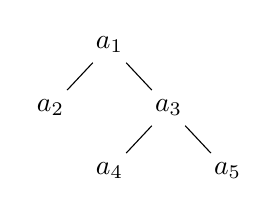
\begin{tikzpicture}[level distance=8mm]
        \node {$a_1$}
            child {node {$a_2$}}
            child {node {$a_3$}
            child {node {$a_4$}}
            child {node {$a_5$}}};
    \end{tikzpicture}
    
    \pause
    Et ce conformement au règle de la méthode des tableaux.
    La construction de cette arbre binaire se fait à priori en $\mathcal{O}(n)$
\end{frame}

\begin{frame}{Alternée - Observations}
    On va faire 3 observations, et on va en déduire un algorithme:
    \begin{itemize}
        \item Si un des litteraux dans une branche gauche (les pairs) ne provoquent aucune contradiction, c'est gagné.
        \item Dans le cas inverse, on doit rechercher plus profond dans l'arbre (parcours de la branche droite)
        \item Et ce ainsi de suite, jusqu'à en déduire un arbre fermé, ou pas
        \item Et ce en prenant aussi en compte les litteraux impairs
    \end{itemize}

    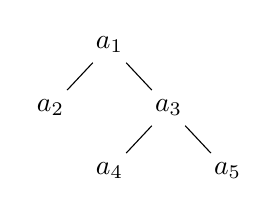
\begin{tikzpicture}[level distance=8mm]
        \node {$a_1$}
            child {node {$a_2$}}
            child {node {$a_3$}
            child {node {$a_4$}}
            child {node {$a_5$}}};
    \end{tikzpicture}
\end{frame}

\begin{frame}{Alternée - Schema Algorithme}
    On décrit un appel de l'algorithme qu'on implémente de manière recursive (dans le cas général):
    Avant cela on créé un dictionnaire. 
    On appelle litteral droit les litteraux impairs et gauche les pairs:  
    \begin{enumerate}
        \item On analyse le litteral droit, si il y a contradiction, l'arbre est fermé, sinon on ajoute eventuellement dans le dictionnaire le litteral
        \item On analyse le litteral gauche, si il produit une contradiction, appel recursif plus profond dans l'arbre, sinon la formule est satisfiable
    \end{enumerate}
    On peut montrer que cette algorithme est en $\mathcal{O}(n)$
\end{frame}

\begin{frame}{Alternée - Conséquence}
    On a donc trouvé un moyen polynomial pour montrer la satisfiabilité d'une forme alternée !!
    \pause
    \begin{itemize}
        \item En effet, ce programme est en $\mathcal{O}(n)$, c'est un parcours linéaire d'une liste chainée, utilisant des opérateurs sur les Hashtbl qu'on peut supposé constant.
        \item On a prouvé la terminaison et la correction du programme:
        \item La correction (preuve faite) est assuré par l'invariant "Toutes les branches déjà traités sont fermés"
        \item La terminaison (preuve faite) est assuré simplement.
    \end{itemize}
\end{frame}

\begin{frame}{Alternée - Conversion}
    On se demande naturellement quelles sont les formules qu'on peut transformer en formule alternée.
    \begin{itemize}
        \item Quand on traduit une forme alternée, on obtient une FNC dont la taille des clauses est strictement croissante.
        \item On peut trouver des contres exemples: par exemple $a_1\lor a_2$ ne pourra pas s'exprimer sous forme alternée (sauf si on fixe un des littéraux)
        \item En convertissant toutes les formules en FNC, seules certaines formules ayant des clauses à taille croissante pourront être reconvertit en forme alternée.
    \end{itemize}
\end{frame}

\begin{frame}{Alternée - Conclusion}
    On décide de tester la vitesse d'execution de mon algorithme contre deux algorithmes de satisfiabilités optimisés: Quine et Coq.
    On utilise un script Python pour générer les mêmes formules pour les différentes structures données demandés par les algorithmes.
    Sur un dataset de 100 formules genere pseudo-aléatoirement, nous avons les résultats suivants:

    \begin{itemize}
        \item \textbf{Alternée:} 0.000493s
        \item \textbf{Quine (avec conversion en CNF):} 0.025874s
        \item \textbf{Quine (sans conversion en CNF):} 0.018691s
    \end{itemize}
    Donc notre algorithme est 50 fois plus rapide sur ce dataset, ce qui n'est pas tellement supprenant.
\end{frame}

\begin{frame}{La logique du 1er ordre}
    \begin{itemize}
        \item On ajoute les quantificateurs $\exists$ et $\forall$
        \item Un ensemble de fonctions de symboles $\mathcal{F}$ qui a des symboles associe un symbole
        \item Un ensemble de relation $\mathcal{R}$ qui a des symboles associe un booléen.
    \end{itemize}
    On note l'arité le nombre d'argument d'une fonction et $X$ les variables.
    \begin{definition}
        On définit les termes $\mathcal{T}(\mathcal{F}, X)$ par induction:
        \begin{itemize}
            \item Tout $x\in X$ est un terme.
            \item Les constantes sont des termes (symbole d'arité 0).
            \item $f(t_1,\dots, t_n)$ est un terme si $f$ est un symbole d'arité $n$ et $t_1,\dots,t_n$ sont des termes.
        \end{itemize}
    \end{definition}
\end{frame}

\begin{frame}{La méthode des tableaux pour logique du 1er ordre}
    On ajoute quatres règles:

    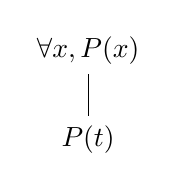
\begin{tikzpicture}[scale=0.75]
    \node {$\forall x, P(x)$}
        child {node {$P(t)$}};
    \end{tikzpicture}
    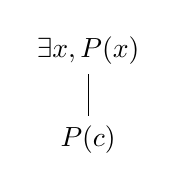
\begin{tikzpicture}[scale=0.75]
    \node {$\exists x, P(x)$}
        child {node {$P(c)$}};
    \end{tikzpicture}
    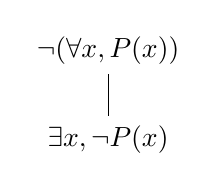
\begin{tikzpicture}[scale=0.75]
    \node {$\lnot(\forall x, P(x))$}
        child {node {$\exists x, \lnot P(x)$}};
    \end{tikzpicture}
    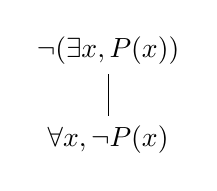
\begin{tikzpicture}[scale=0.75]
    \node {$\lnot(\exists x, P(x))$}
        child {node {$\forall x, \lnot P(x)$}};
    \end{tikzpicture}
    
    où $t$ et $c$ est une variable fixe quelquonque.
    
    \textbf{Attention:} Pour la règle $\forall$, on peut choisir $t$, pour la règle $\exists$, on prend une variable fraiche $c$!
\end{frame}

\begin{frame}{La logique temporelle du temps linéaire}
    \begin{definition}[Formule de la LTL]
        On définit $F$ l'ensemble des formules de la LTL inductivement par:
        \begin{itemize}
            \item $p\in AP \implies p\in F$
            \item si $\psi$ et $\phi$ sont des formules de LTL alors $\lnot\psi, \phi\lor\psi, X\psi, \phi U\psi$ sont des formules de LTL
        \end{itemize}
        $AP$ un ensemble fini de variables propositionnelles.
    \end{definition}
    \begin{definition}[Opérateurs X et U]
            \begin{itemize}
                \item $X\phi$ : $\phi$ doit être satisfaite dans l'état suivant (neXt)
                \item $\psi U\phi$ : $\psi$ doit être satisfaite dans tous les états jusqu'à un état où $\phi$ est satisfait (Until)
            \end{itemize}
        \end{definition}
\end{frame}

\begin{frame}{Etat dans la LTL}
    \begin{definition}[Monde]
        On définit un tel objet comme $\omega := w_0,w_1,\dots$ une suite infinie d'état.
        On écrira $\omega^i:=w_i,w_{i+1},\dots$ un suffixe de $\omega$.
    \end{definition}
    Soit $v : \omega\times F \rightarrow \{T,F\}$ une fonction de valuation.
    \begin{definition}[Satisfaction d'un monde]
        En LTL, on définit $\omega \models f$ via:
        \begin{itemize}
            \item $\omega \models a$ si $v(w_0,a) = T$ si $a$ atomique 
            \item $\omega \models \lnot f$ si $\lnot(\omega \models f)$ 
            \item $\omega \models f\lor g$ si $\omega \models f$ ou $\omega \models g$
            \item $\omega \models \textbf{X}f$ si $\omega^1 \models f$
            \item $\omega \models f\textbf{U}g$ si $\omega \models g$ ou $\omega \models f\land\textbf{X}(f\textbf{U}g)$
        \end{itemize}
    \end{definition}
\end{frame}

\begin{frame}{Méthode des tableaux en LTL}
    On définit deux nouvelles règles pour la méthode des tableaux en LTL:

    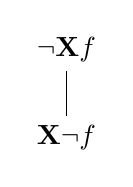
\begin{tikzpicture}[scale=0.75]
    \node {$\lnot\textbf{X}f$}
        child {node {$\textbf{X}\lnot f$}};
    \end{tikzpicture}
    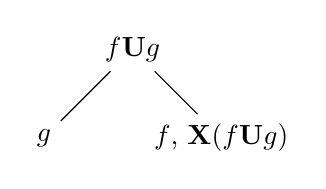
\begin{tikzpicture}[scale=0.75, level 1/.style={sibling distance=3cm}]
    \node {$f\textbf{U}g$}
        child {node {$g$}}
        child{node {$f$, $\textbf{X}(f\textbf{U}g)$}};
    \end{tikzpicture}
    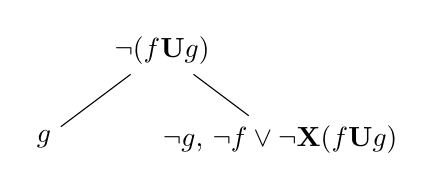
\begin{tikzpicture}[scale=0.75, level 1/.style={sibling distance=4cm}]
    \node {$\lnot(f\textbf{U}g)$}
        child {node {$g$}}
        child{node {$\lnot g$, $\lnot f \lor \lnot\textbf{X}(f\textbf{U}g)$}};
    \end{tikzpicture}

    \begin{definition}[Formule élementaire]
        $f$ est élementaire ssi il respecte un de ses 2 points:
        \begin{itemize}
            \item C'est une formule atomique (ou la négation d'une formule atomique)
            \item Il a comme connecteur logique "principale" $\textbf{X}$ (des X-formules)
        \end{itemize}
    \end{definition}
    Si un noeud contient uniquement des formules elementaires, alors on créé un fils
    du noeud contenant toutes les \textbf{X}-formules sans leur connecteur logique principal $\textbf{X}$
\end{frame}

\begin{frame}{Exemples d'utilisation de la méthode des tableaux}
    On peut trouver plusieurs applications à la LTL et à la méthode des tableaux:
    \begin{itemize}
        \item Preuve de programme concurrentiel
        \item Raisonnement sur des circuits intégrés
        \item Raisonnement sur les protocoles de communications
    \end{itemize}
    Toutes ces applications s'inscrivent dans le cadre de la vérification de modèles qui est une méthode permettant de montrer
    la correction de systèmes informatiques complexes.

\begin{definition}[Verification de modèle (Model Checking)]
    Technique de vérification qui explore tout les états possible d'un système de manière force brute.
\end{definition}
\end{frame}


\begin{frame}{A propos du model checking}
    \begin{itemize}
        \item Ce n'est pas avec la LTL que nous allons faire des gros exemples de model checking (Un model checker de base peut s'occuper de $10^9$ états environ, allant jusqu'à $10^{476}$ pour les meilleurs!).
        \item Ainsi un model checker typique pourrait utiliser entre autres la LTL pour s'occuper en particulier des deadlocks. C'est ainsi qu'on pourrait utiliser la méthode des tableaux pour prouver une formule qui montre
            que des algorithmes vont bien s'executer de manière à ne pas avoir d'inter-dépendance.
        \item Ainsi nous allons examiner un exemple dans lequel nous allons appliquer la méthode des tableaux pour prouver le bon fonctionnement du système choisit!
    \end{itemize}    
\end{frame}

\begin{frame}{Automate de Büchi}
Un automate de Büchi est un 5-uplets $(S, I, T, F, \Sigma)$ tel que
\begin{itemize}
    \item $S$ est un ensemble fini d'état
    \item $I\subseteq S$ un ensemble d'état initiaux
    \item $F\subseteq S$ un ensemble d'état finaux
    \item $\Sigma$ Un ensemble fini de symboles appelé alphabet
    \item $T: \{S\times \Sigma\}\mapsto \mathcal{P}(S)$ Une fonction de transition.
\end{itemize}
Cet automate particulier accepte des séquences infinis (donc des mots infinis) ssi le mot passe par un état acceptant une infinité de fois.
C'est un outil utilisé dans le cadre de la vérification de modèle en LTL.
\end{frame}

\begin{frame}{Büchi en LTL}
    On va utiliser l'algorithme de Gerth pour transformer notre formule LTL en Automate de Büchi Généralisé (GBA)
    \begin{definition}[GBA]
        Un GBA est un automate de Büchi avec la seule particularité que $F$ est un ensemble d'ensemble d'état acceptant appelé \textbf{condition d'acceptation}.
        
        Un GBA accepte un mot ssi il est passé au moins une fois par un état dans chaque ensemble d'état acceptant.
    \end{definition}
    Nous nous ramenerons à un Automate de Büchi via un autre algorithme pour simplifier.
\end{frame}

\begin{frame}{Notre But}
Résolution par Tableau et par Buchi (après implémentation des solutions). Comparaison des algorithmes en terme de rapidité ? 
\end{frame}

\begin{frame}{Contexte}
Application, un simple feu rouge ?
\end{frame}

\begin{frame}{Bibliographie}
\begin{enumerate}
    \item Logique: fondements et applications (Dunod) de Pierre Le Barbenchon, Sophie Pinchinat, François Schwarzentruber
    \item Mathematical Logic: Tableaux Reasoning for Propositional Logic de Chiara Ghidini (https://dit.unitn.it/~ldkr/ml2015/slides/PLtableau.pdf)
    \item Tableau Methods for Propositional Logic and Term Logic de Tomasz Jarmużek
    \item The tableau method for temporal logic: an overview - Pierre WOLPER
    \item Principles of Model Checking - Christel Baier et Joost-Pieter Katoen
\end{enumerate}
\end{frame}

\begin{frame}[fragile]{Code - Méthode des tableaux classique 1}
    \begin{center}
        \begin{tabular}{c}
            \begin{lstlisting}
                type formula =
                    | Atom of string
                    | Not of formula
                    | And of formula * formula
                    | Or of formula * formula

                let rec expand formula =
                    match formula with
                    | Not (Not f) -> [[f]]
                    | Not (And (f1, f2)) -> [[Not f1]; [Not f2]]
                    | Not (Or (f1, f2)) -> [[Not f1; Not f2]]
                    | And (f1, f2) -> [[f1; f2]]
                    | Or (f1, f2) -> [[f1]; [f2]]
                    | _ -> [];;

                let rec has_cycle branch =
                    List.exists (fun f -> List.mem (Not f) branch) branch;;
            \end{lstlisting}
        \end{tabular}
      \end{center}
\end{frame}

\begin{frame}[fragile]{Code - Méthode des tableaux classique 2}
    \begin{center}
        \begin{tabular}{c}
            \begin{lstlisting}
                let rec tableau branches =
                    match branches with
                    | [] -> false
                    | branch :: rest -> 

                    if has_cycle branch then
                        tableau rest
                    else
                        match branch with
                        | [] -> true
                        | f :: fs ->

                        let expansions = expand f in match expansions with
                        | [] -> tableau (fs :: rest)
                        | new_branches ->
                        
                        let expanded_branches = List.map (fun b -> b @ fs) new_branches in
                        tableau (expanded_branches @ rest);;

                    let is_satisfiable formula =
                    let initial_branch = [formula] in tableau [initial_branch];;
            \end{lstlisting}
        \end{tabular}
    \end{center}
\end{frame}

\begin{frame}[fragile]{Code - Méthode des tableaux classique 1}
    \begin{center}
        \begin{tabular}{c}
            \begin{lstlisting}
                type prop = | Var of string | Not of prop | And of prop * prop | Or  of prop * prop
                (* Une branche c'est une liste de formule avec un signe *)
                type branch =  (bool * prop) list

                let is_literal = function
                    | (true, Var _) -> true
                    | (false, Var _) -> true
                    | (true, Not (Var _)) -> true
                    | (false, Not (Var _)) -> true
                    | _ -> false
            
                (* Check les contradictions *)
                let branch_closed (br : branch) : bool =
                    let pos = Hashtbl.create 16 in
                    let neg = Hashtbl.create 16 in
                    let record = function
                        | (true, Var v) -> Hashtbl.replace pos v true
                        | (false, Var v) -> Hashtbl.replace neg v true
                        | (true, Not (Var v)) -> Hashtbl.replace neg v true
                        | (false, Not (Var v)) -> Hashtbl.replace pos v true
                        | _ -> ()
                    in
                    List.iter record br;
                    let closed = ref false in
                    Hashtbl.iter (fun v _ -> if (Hashtbl.mem pos v) && (Hashtbl.mem neg v) then closed := true) pos;
                    !closed
            \end{lstlisting}
        \end{tabular}
      \end{center}
\end{frame}

\begin{frame}[fragile]{Code - Méthode des tableaux classique 2}
    \begin{center}
        \begin{tabular}{c}
            \begin{lstlisting}
            (* La decomposition usuelle faites durant la methode des tableaux *)
            let decompose_once (br : branch) : branch list option =
                let rec find_nonlit acc = function
                    | [] -> None
                    | x :: xs ->
                    if is_literal x then find_nonlit (x::acc) xs
                    else Some (List.rev acc, x, xs)
                in
                match find_nonlit [] br with
                | None -> None
                | Some (left, (sign, form), right) ->
                    let rest = left @ right in
                    let mk b p = (b, p) in
                    (match sign, form with
                    | true, And (a,b) ->
                    Some [ (mk true a) :: (mk true b) :: rest ]
                    | false, Or (a,b) ->
                    Some [ (mk false a) :: (mk false b) :: rest ]
                    | true, Or (a,b) ->
                    Some [ (mk true a)::rest; (mk true b)::rest ]
                    | false, And (a,b) ->
                    Some [ (mk false a)::rest; (mk false b)::rest ]
                    | true, Not a ->
                    Some [ (mk false a) :: rest ]
                    | false, Not a ->
                    Some [ (mk true a) :: rest ]
                    | _, _ -> None)
            \end{lstlisting}
        \end{tabular}
    \end{center}
\end{frame}


\begin{frame}[fragile]{Code - Méthode des tableaux classique 3}
    \begin{center}
        \begin{tabular}{c}
            \begin{lstlisting}
                (* La Methode des Tableaux en soit *)
                let satisfiable (phi : prop) : bool =
                let initial_branch = [ (true, phi) ] in
                let rec explore_stack stack =
                    match stack with
                    | [] -> false
                    | br :: rest ->
                    if branch_closed br then explore_stack rest else
                    match decompose_once br with
                    | None -> true
                    | Some new_branches -> explore_stack (new_branches @ rest)
                    in explore_stack [ initial_branch ]
            \end{lstlisting}
        \end{tabular}
    \end{center}
\end{frame}

\begin{frame}[fragile]{Code - Alternée 1}
    \begin{center}
        \begin{tabular}{c}
            \begin{lstlisting}
                type formula =
                    | Atom of (string* bool)
                    | And of (string*bool) * formula
                    | Or of (string*bool) * formula

                type branch = 
                    | Empty
                    | Node of (formula option * formula * branch);;

                let extract (f:formula option) = match f with
                    | None ->  Atom("none", false)
                    | Some t -> t

                let rec print_formula (f:formula) = match f with
                    | Atom(s, b) -> if b then print_string s else print_string "Not ";print_string s;
                    | And ((f, b),g) -> if b then print_string f else print_string "Not ";print_string f;print_string " And ";print_formula g
                    | Or ((f,b),g) -> if b then print_string f else print_string "Not ";print_string f;print_string " Or ";print_formula g;;

                let rec print_branches (b:branch) =
                    print_string " [";
                    match b with
                        | Empty -> ()
                        | Node(a1, a2, b) -> print_formula@@extract a1;print_string ", ";print_formula a2;print_branches b;
                    print_string "]";; 
            \end{lstlisting}
        \end{tabular}
    \end{center}   
\end{frame}

\begin{frame}[fragile]{Code - Alternée 2}
    \begin{center}
        \begin{tabular}{c}
            \begin{lstlisting}
            let rec formula2branch (f:formula) : branch = match f with
                | And(a, Or(b, Atom(c))) -> Node(Some(Atom b), Atom a, Node(None, Atom(c), Empty))
                | And(a, Or(b, c)) ->  Node(Some(Atom b), Atom a, formula2branch c)
                | And(a, Atom(b)) -> Node(Some (Atom b), Atom a, Empty)
                | _ -> failwith "Pas alternee"
              
            let has_cycle (br:branch) : bool = 
                let rec aux (br:branch) (d:(string,bool) Hashtbl.t) : bool = match br with
                | Node(None, Atom (f, b), Empty) -> 
                  if Hashtbl.mem d f then 
                    Hashtbl.find d f = b
                  else
                    true
                | Node(Some(Atom(fg, bg)), Atom (fd, bd), Empty) -> 
                      if Hashtbl.mem d fd then
                        if Hashtbl.find d fd = bd then
                          not @@ Hashtbl.mem d fg && Hashtbl.find d fg <> bg
                        else 
                          false
                      else(
                        Hashtbl.add d fd bd;
                        not @@ Hashtbl.mem d fg && Hashtbl.find d fg <> bg)
                | Node(Some (Atom (fg, bg)), Atom (fd, bd), nb) ->
                  if Hashtbl.mem d fd then
                    if Hashtbl.find d fd <> bd then
            \end{lstlisting}
        \end{tabular}
    \end{center}   
\end{frame}

\begin{frame}[fragile]{Code - Alternée 3}
    \begin{center}
        \begin{tabular}{c}
            \begin{lstlisting}
                        false
                            else
                            if Hashtbl.mem d fg then
                                if Hashtbl.find d fg = bg then
                                true
                                else
                                aux nb d
                            else
                                true
                        else
                            (Hashtbl.add d fd bd;
                            if Hashtbl.mem d fg then
                            if Hashtbl.find d fg = bg then
                                true
                            else
                                aux nb d
                            else
                            true)
                        | _ -> failwith "Pas alternee"
                        in aux br (Hashtbl.create 100);;
          
                        let is_satisfiable (f:formula) : bool = let b = formula2branch f in has_cycle b;;
            \end{lstlisting}
        \end{tabular}
    \end{center}   
\end{frame}
\end{document}